% Offizielle Beispieldatei für beamer-Vorlage aus tubslatex Version 0.3beta2
\documentclass[fleqn,11pt,aspectratio=169]{beamer}

\usepackage[ngerman]{babel}
\usepackage[utf8x]{inputenc}
\usepackage{graphicx}
\usepackage{tikz}
\usepackage{pgfplots}

\usetheme[%
  %nexus,%        Nexus Fonts benutzen
  %lnum,%         Versalziffern verwenden
  %cmyk,%<rgbprint>,          Auswahl des Farbmodells
  blue,%<orange/green/violet> Auswahl des Sekundärfarbklangs
  dark,%<light,medium>        Auswahl der Helligkeit
  %colorhead,%    Farbig hinterlegte Kopfleiste
  %colorfoot,%    Farbig hinterlegt Fußleiste auf Titelseite
  colorblocks,%   Blöcke Farbig hinterlegen
  %nopagenum,%    Keine Seitennumer in Fußzeile
  %nodate,%       Kein Datum in Fußleiste
  tocinheader,%   Inhaltsverzeichnis in Kopfleiste
  %tinytocinheader,% kleines Kopfleisten-Inhaltsverzeichnis
  %widetoc,%      breites Kopfleisten-Inhaltsverzeichnis
  %narrowtoc,%    schmales Kopfleisten-Inhaltsverzeichnis
  %nosubsectionsinheader,%  Keine subsections im Kopfleisten-Inhaltsverzeichnis
  %nologoinfoot,% Kein Logo im Fußbereich darstellen
  ]{tubs}

% Titelseite
\title{Multi-Lane Standards and Techniques for 100/400 Gigabit Ethernet}
\subtitle{An brief overview}
\author{Christoph Seitz}
% Titelgrafik, automatisch beschnitten, Weitere Optionen: <scaled/cropx/cropy>
% \titlegraphic[cropped]{\includegraphics{infozentrum.jpg}}
\titlegraphic[scaled]{\includegraphics{titlepicture.jpg}}

% Logo, dass auf Titelseiten oben rechts und auf Inthaltsseiten unten rechts
% dargestellt wird. Es wird jeweils automatisch skliert
%\logo{\includegraphics{dummy_institut.pdf}}
%\logo{Institut für Unkreativität\\und Schreibschwäche}

\begin{document}

\begin{frame}[plain]
\titlepage
\end{frame}

\begin{frame}[highlight]{Agenda}
\tableofcontents
\end{frame}

\section{Introduction}

%http://www.cisco.com/c/en/us/solutions/collateral/service-provider/ip-ngn-ip-next-generation-network/white_paper_c11-481360.html
\begin{frame}{Motivation}
\begin{itemize}
  \item IP traffice will grow 21 \% per year from 2013 to 2018
  \item Demand for higher bandwidth
  \begin{itemize}
    \item Storage Area Networks
    \item Distributed Data Warehouses
    \item Content Delivery
  \end{itemize}
  \item Faster server connections
  \item Faster switch interconnects
\end{itemize}
\end{frame}

\begin{frame}{Development of the IEEE 802.3 Ethernet Standard}
\begin{tikzpicture}
\begin{semilogyaxis}[height=\textheight,width=\textwidth,xlabel=year,ylabel=data rate in b/s,
xtick={1985,1990,...,2015},
xmin=1980,
xmax=2020,
ymin=1000000,
ymax=1000000000000,
axis x line=bottom,
axis y line=left,
/pgf/number format/.cd,set thousands separator={}]
\addplot[nodes near coords,mark=*,point meta=explicit symbolic] table[row sep=crcr,meta=label] {
 x y label\\
1983 10000000 10Mb\textbackslash s\\
1995 100000000 100Mb\textbackslash s\\
1998 1000000000 1Gb\textbackslash s\\
2002 10000000000 10Gb\textbackslash s\\
2010 100000000000 100Gb\textbackslash s\\
2017 400000000000 400Gb\textbackslash s\\
};
\end{semilogyaxis}
\end{tikzpicture}

\end{frame}

\section{Techniques for 100/400 Gigabit Ethernet}
\subsection{Overview}
\begin{frame}{Overview}
\begin{columns} % align columns
\begin{column}{.6\textwidth}
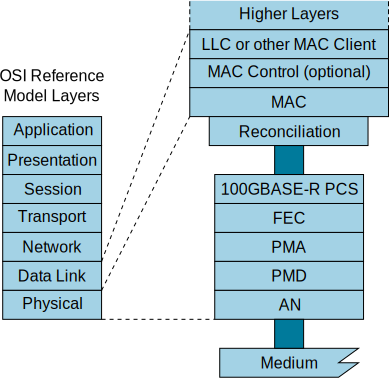
\includegraphics[height=.95\textheight]{overview.pdf}
\end{column}
\begin{column}{.4\textwidth}
\begin{itemize}
\item Data endcoding and multi-lane distribution
\item Lane deskwes
\item Bit-level mutiplexing and toleration of skew variation
\item Physical Mediums
\item Forward error correction
\end{itemize}
\end{column}
\end{columns}
\end{frame}

\subsection{Physical Coding Sublayer}
\begin{frame}{The Physical Coding Sublayer}
\begin{columns} % align columns
\begin{column}{.6\textwidth}
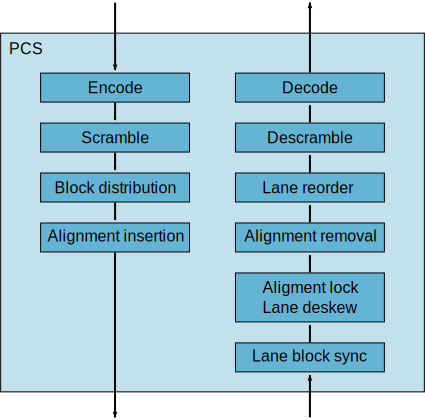
\includegraphics[height=0.95\textheight]{pcs.pdf}
\end{column}
\begin{column}{.4\textwidth}
\begin{itemize}
\item Each lane runs at 10.3125 Gb\textbackslash s
\item 64b/66b encoding and decoding
\item Multi-lane distribution
\item Marker insertion and removal
\item Lane deskew and reorder
\item Lane Block sync and alignment lock
\end{itemize}
\end{column}
\end{columns}
\end{frame}

\begin{frame}{Multi-lane distribution and alignment marker insertion}
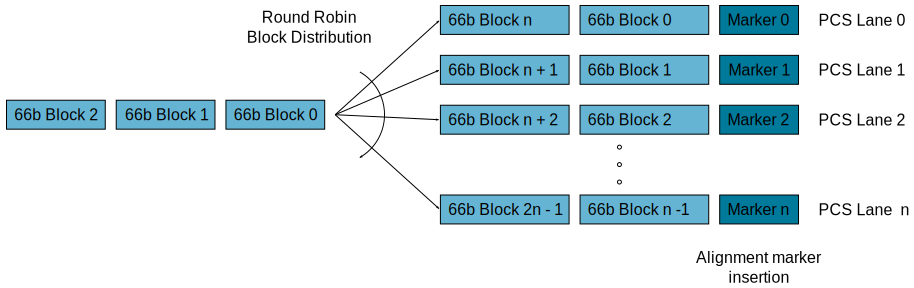
\includegraphics[width=\linewidth]{mld.pdf}

\end{frame}

\subsection{Physical Medium Attachment}

\subsection{Physical Medium Dependent sublayer}
\subsection{Forward error correction}
\begin{frame}{Forward error correction}
\begin{itemize}
\item  Needed to support a BER  of $10^{-12}$ or better
\item FEC code used is a cyclic code (2112, 2080) for error checking and forward error correction
\item Corrects an error burst of up to 11 bits per block
\item Compresses the sync header of an 66b PCS to gain space 32 parity bits
\item Calculates the code word and then scramble it again
\item Required for 100G when copper cables and backplanes are used
\end{itemize}
\end{frame}

\section{Outlook}
\subsection{400 Gb\textbackslash s Ethernet}
\begin{frame}{400 Gb\textbackslash s Ethernet}
\begin{itemize}
  \item Keep the general design of 40/100 Gb\textbackslash s standard
  \item Extend PCS to 16 Lanes and operate at 25.78125 Gb\textbackslash s
  \item Require Read-Solomon FEC for BER better than or equal to $10^{-13}$
  \item Possible use pulse-amplitude modulation (PAM-4) for signal modulation
  \item Various speed, lane counts and modulation are possible
  \item Still a topic in research and development
\end{itemize}
\end{frame}

\end{document}
